The 2022 fieldwork involved 2 separate teams
conducting parallel missions -- one for the rover side and one for the drone side.
In subsequent fieldwork sessions, the teams will run a joint mission.
The missions are organized in a set of simulated ``sols'' -- a word designating a day in the context
of some particular planet, abstracting from the 24-hour period implied by an Earth day.
The goal of the 3-week fieldwork is to carry out approximately 10 sols,
under the assumption that about 40\% of the days will be rained out
and that people will need some days off (during which they typically head out to Myvatn).
Multiple sols can be simulated in a single day.

Each team in the fieldwork is divided into 3 groups:
\begin{itemize}
	\item \textbf{Implementation:} these are the people who physically carry out data collection,
	drive the rover, fly the drones, collect hyperspectral data, 
	collect Laser Induced Breakdown Spectroscopy (LIBS) data, take samples of rock/sand,
	and -- perhaps most importantly -- \emph{document} everything that happens.
	\item \textbf{Operations:} these are the people who give orders to the implementation team,
	telling them where to take samples, and giving them mission goals,
	e.g.~``take a survey from this coordinate A to coordinate B.''
	The operations team also receives and analyzes data from the field (and forward it to offsite
	team members) in order to inform subsequent missions.
	They are not allowed to go to the implementation site, nor to read/ask about it.
	It should appear as a black box to them, as would the Martian surface site.
	\item \textbf{Offsite:} these are not in the field but participate in data analysis
	and determination of high-level mission goals.
\end{itemize}

\subsection{Heli}
The thin Martian atmosphere means that it is inefficient to use typical multirotor drones for
Martian exploration.
Helicopters' large, slow-moving rotors create thrust create thrust more efficiently in a scenario
where energy is a precious resource.
However, in the recent past, much more earth-based research effort into UAS (uncrewed aerial systems)
has gone into multirotor drones.
Multirotor drones have fewer moving physical parts, and are simpler products for consumers
and industry to use.
For this simulation, where the goal is to test the mission operations themselves,
the details are not as important, and the large helicopters are therefore replaced by easier-to-use
multirotor drones.

A typical drone mission will include a flight, survey, and data collection with one or more operations
after landing (possibly on a different sol, to simulate the time required for recharging).
Such operations can include drilling, picking things up with a claw, analyzing chemical composition
of the ground beneath the drone, and taking pictures of the landing site.

\begin{figure}
	\centering
	\begin{subfigure}{0.49\textwidth}
	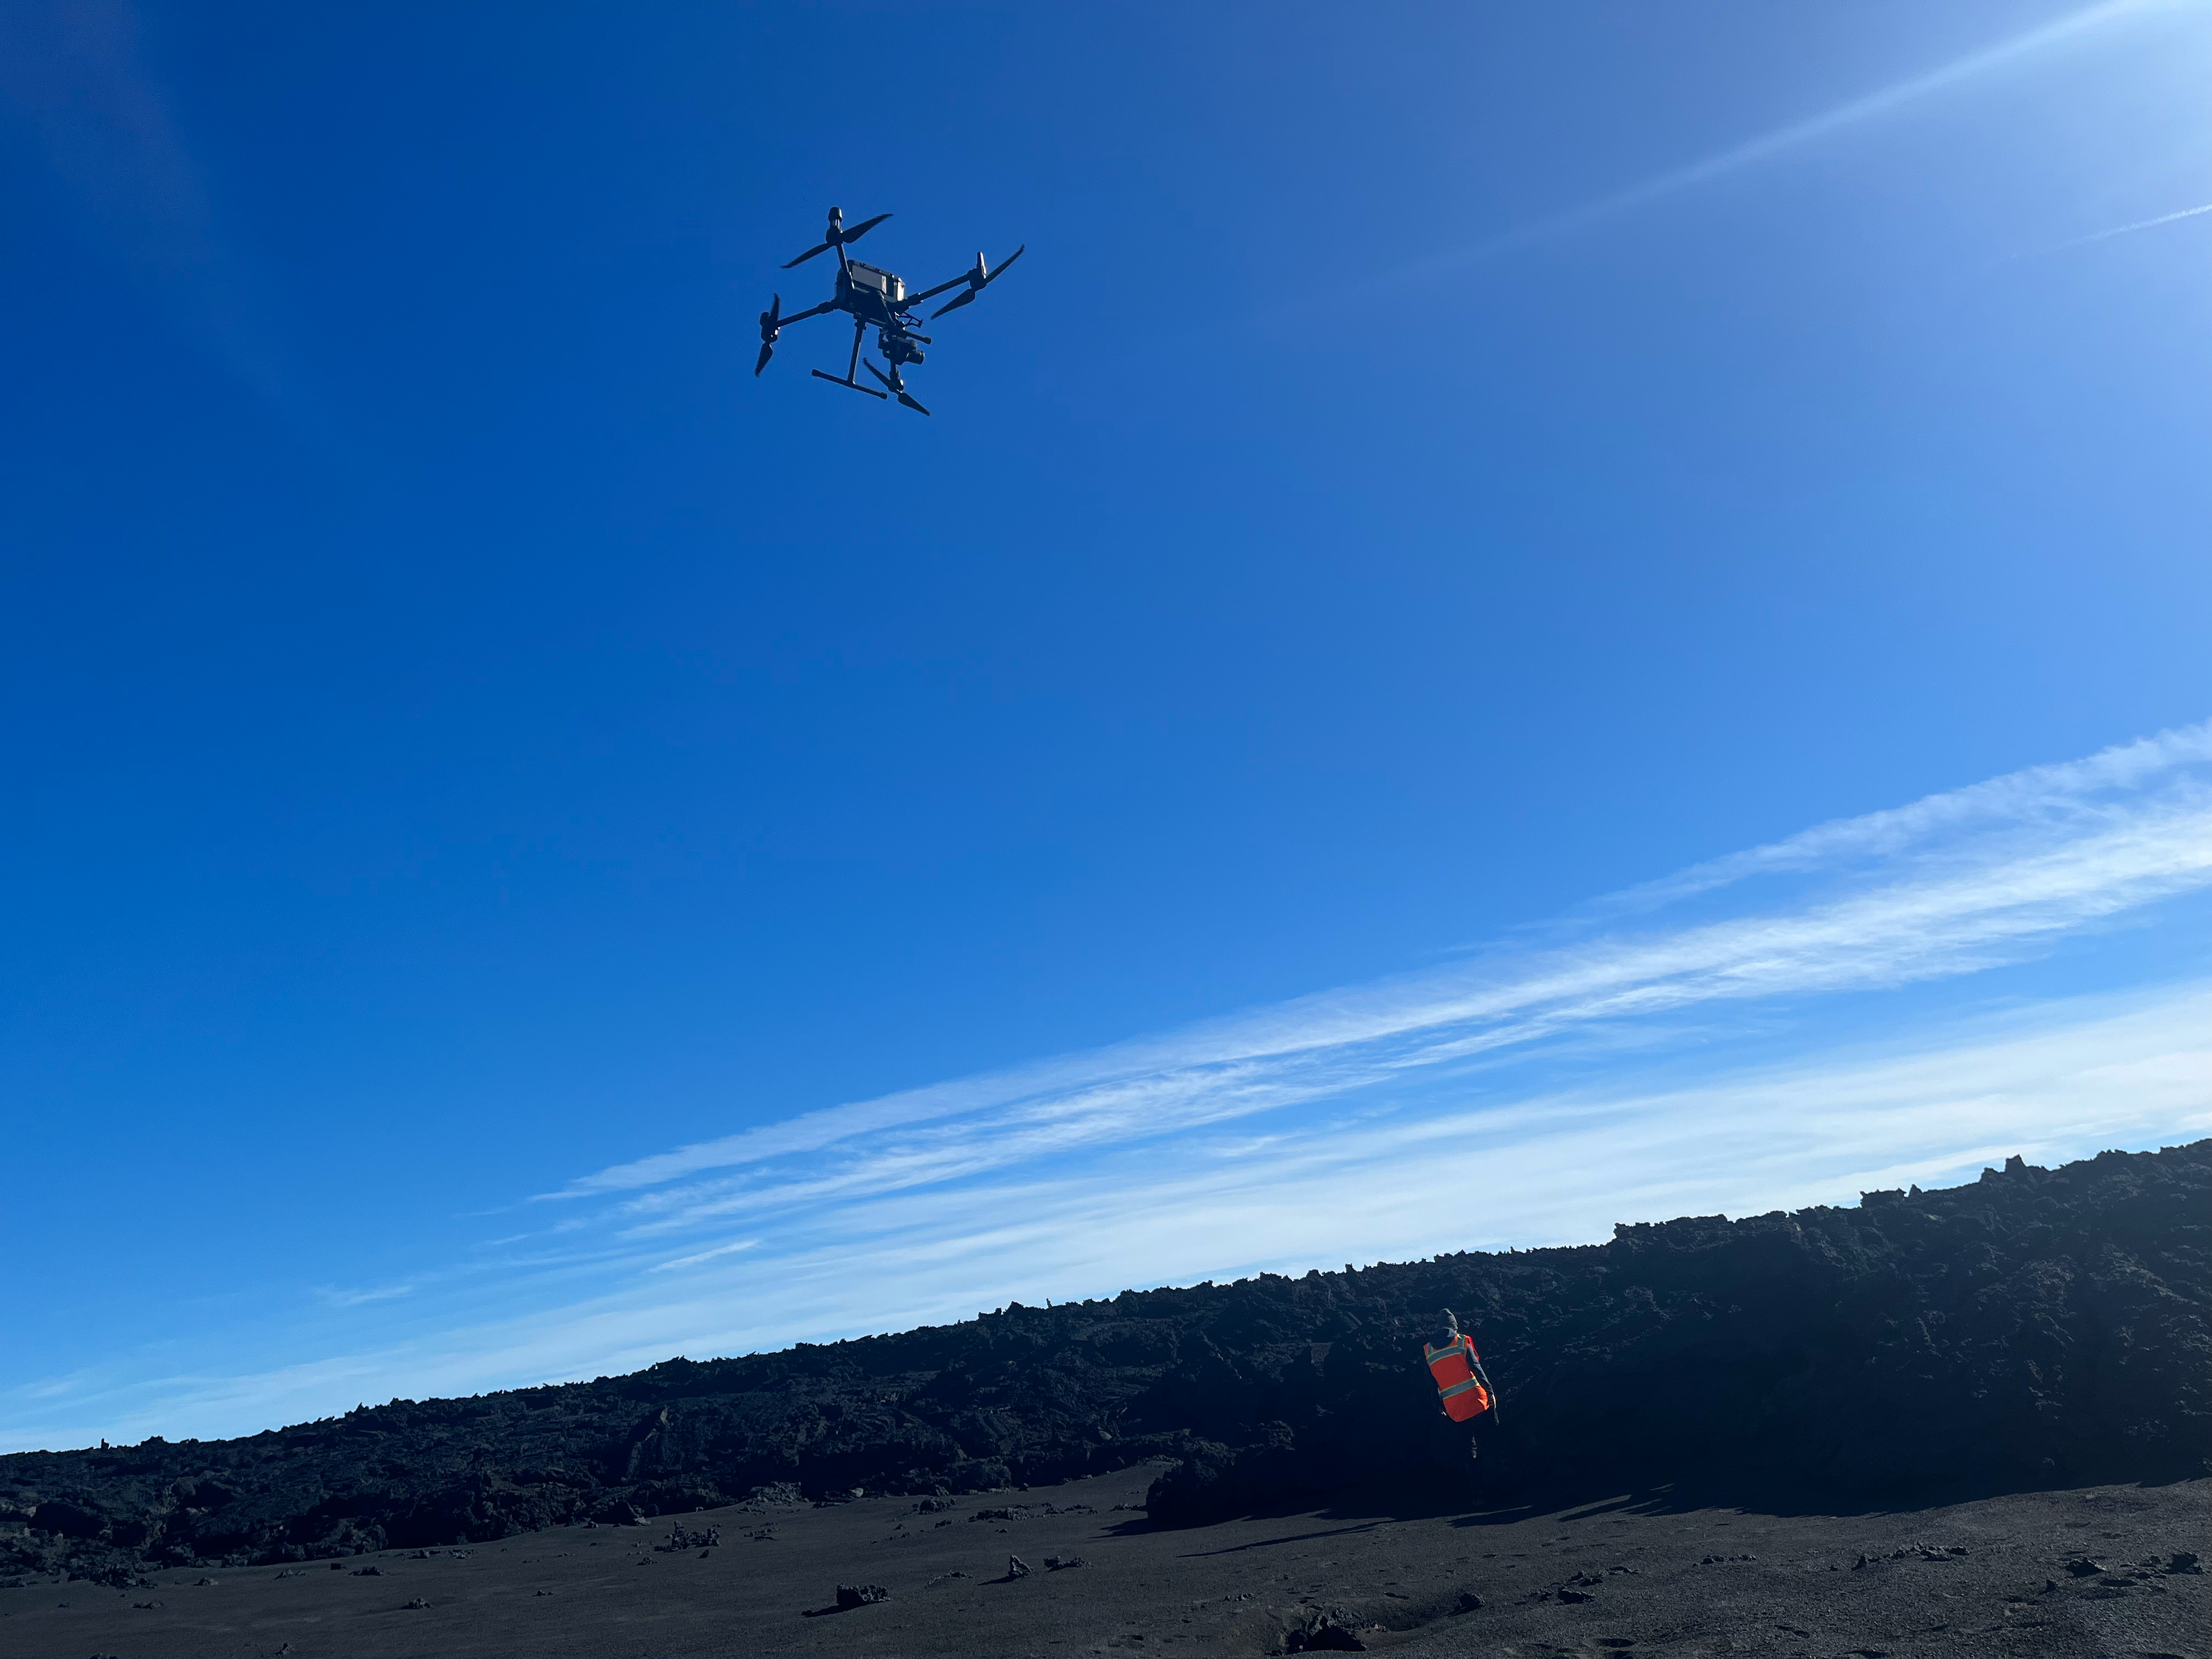
\includegraphics[width=\textwidth]{./images/matrice_holuhraun.png}
	\caption{A DJI matrice flying above Holuhraun.}
	\label{figure:matrice_holuhraun}
	\end{subfigure}
	\centering
	\begin{subfigure}{0.49\textwidth}
	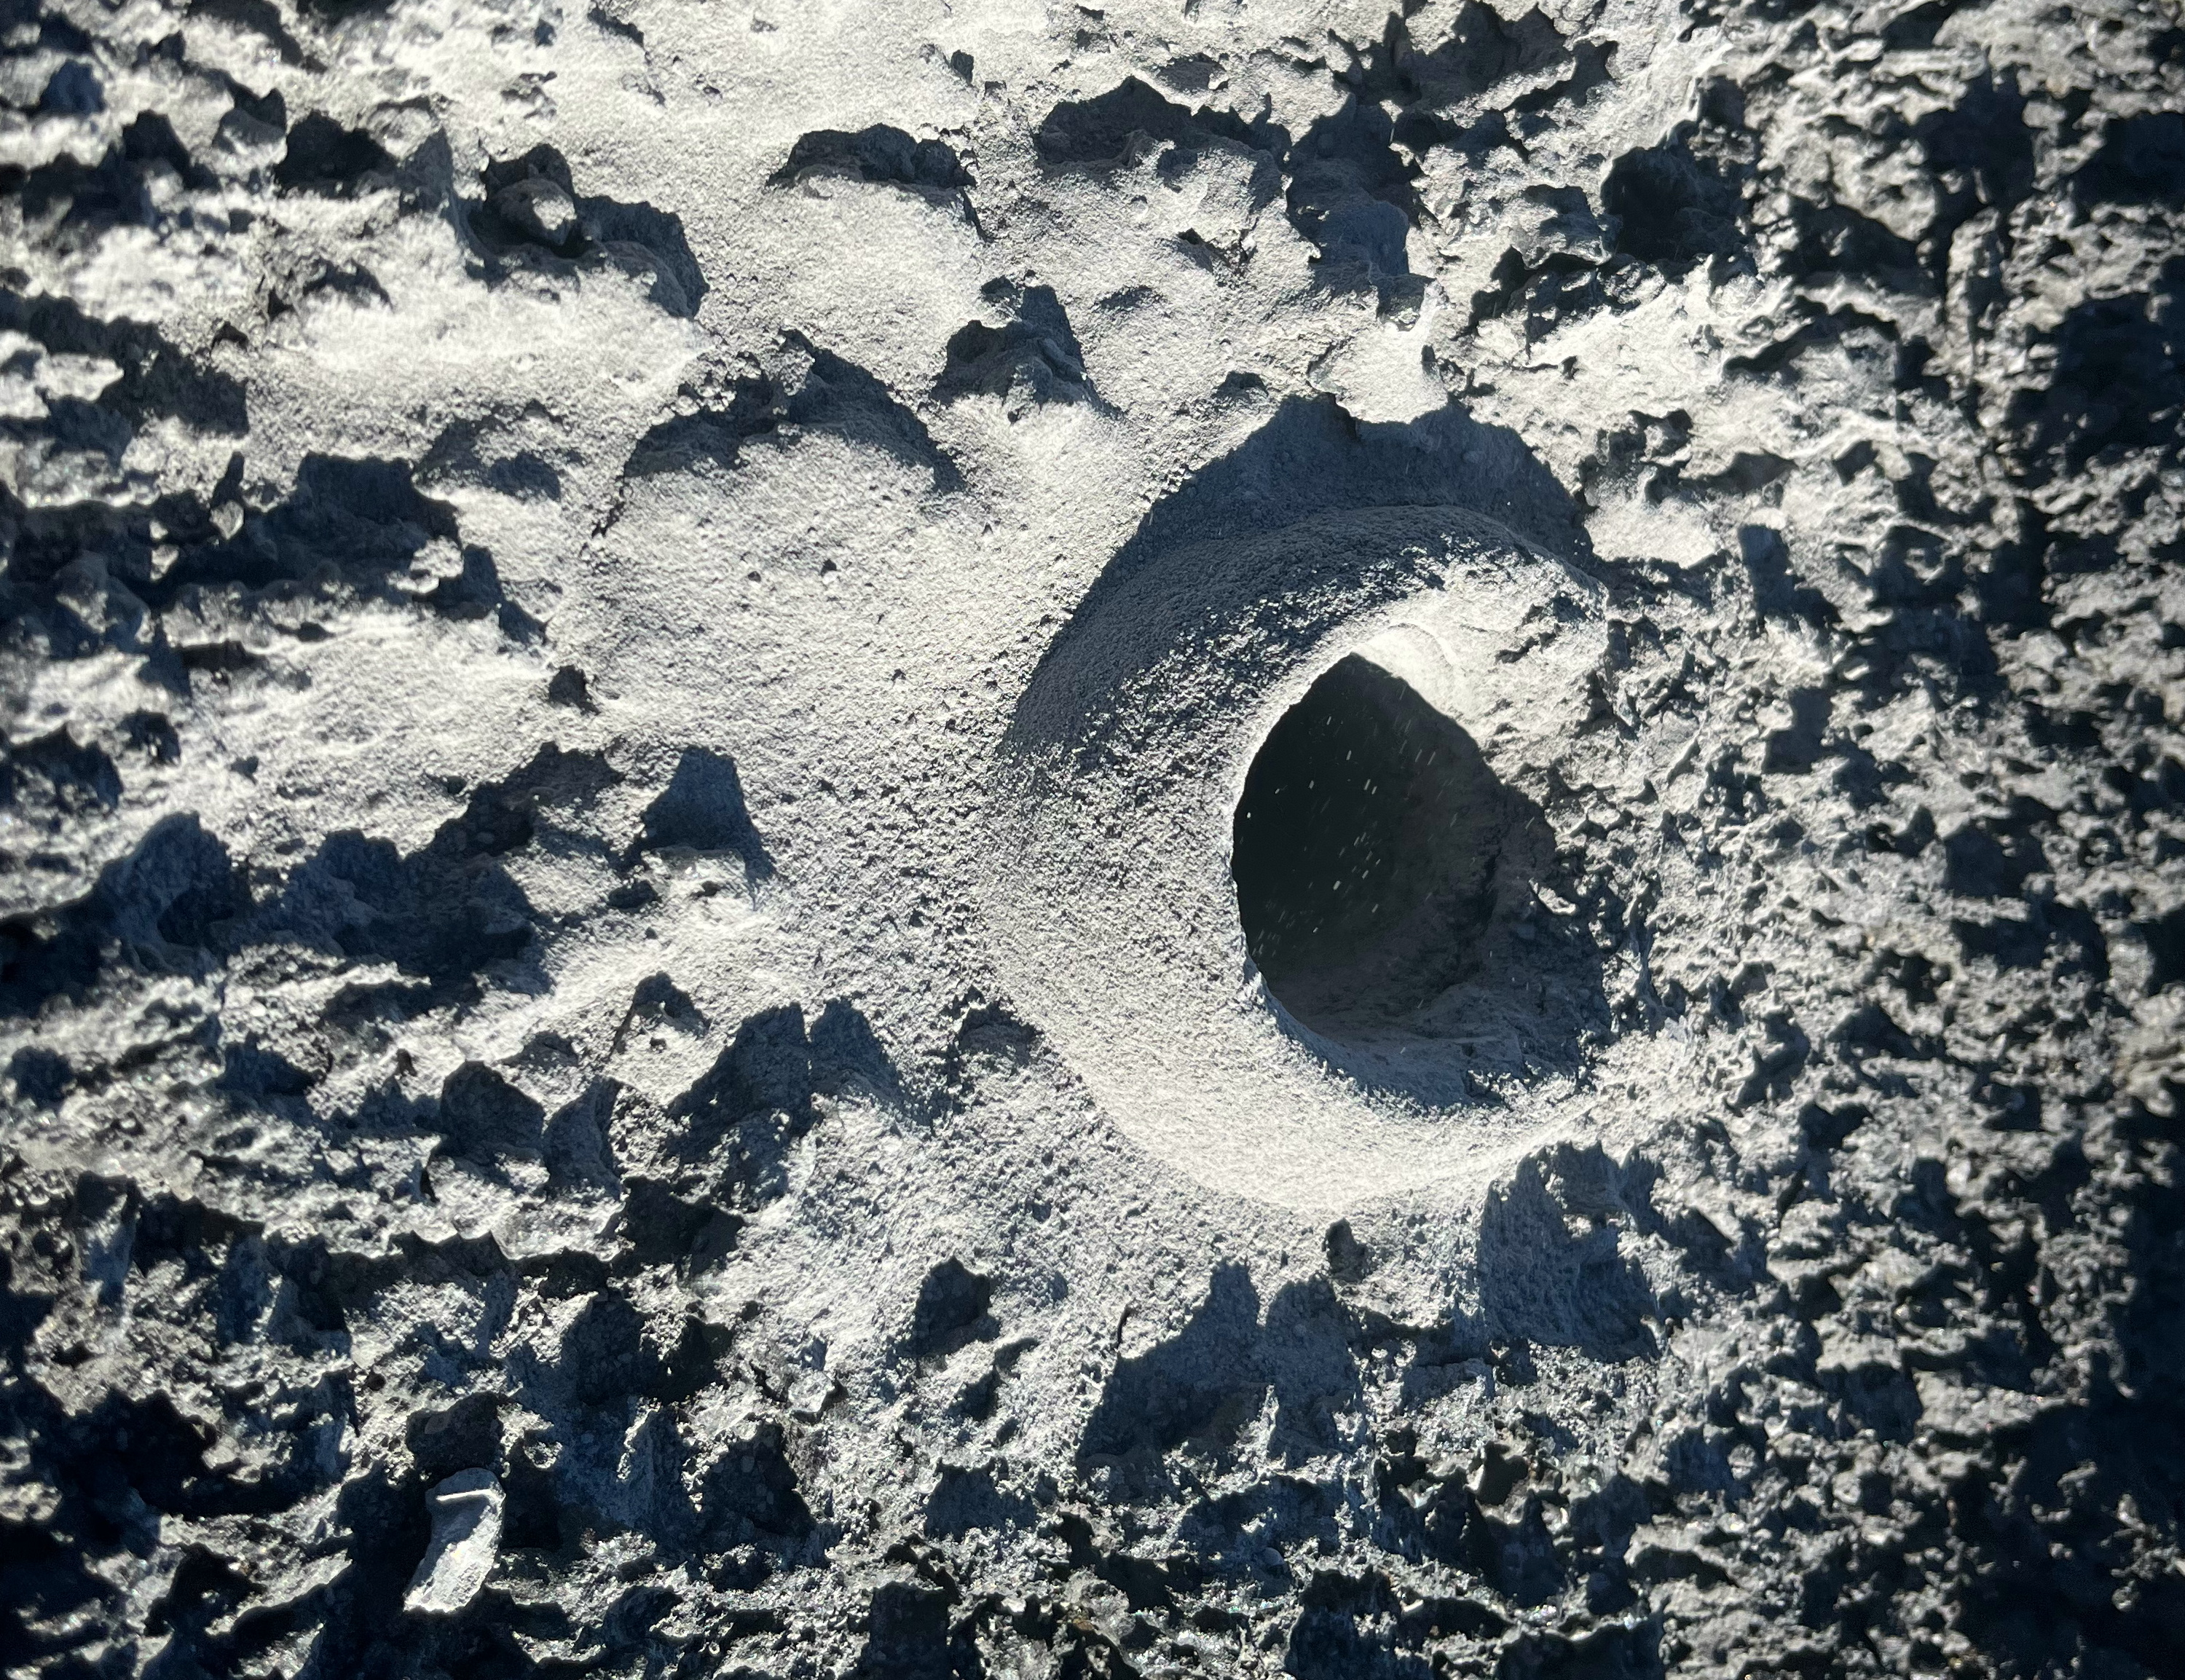
\includegraphics[width=\textwidth]{./images/heli_drill_site.png}
	\caption{A drill site on the lava flow.}
	\label{figure:heli_drill_site}
	\end{subfigure}
	\caption{Some heli implementation}
	\label{figure:heli_implementation}
\end{figure}

\subsection{Rover}
RAVEN has a replica of a Mars rover from the Canadian Space Agency, called MESR.

